
%%----------------------------------------------------
\section{Introduction} \label{sec:intro}
%%----------------------------------------------------

Solar flares are the largest magnetic events within our solar system. They are characterized by the sudden release of magnetic energy, leading to localized, transient heating of coronal plasma to temperatures exceeding approximately 10 million Kelvin (MK), significantly hotter than the surrounding coronal plasma at around 1 MK. Flares are typically identified by the peak soft X-ray flux observed by the X-Ray Sensor onboard the Geostationary Operational Environmental Satellites (GOES/XRS), often referred to as the "GOES class" \citep{xrs}. Flares classified as GOES class C and above typically heat the coronal plasma to temperatures ranging from 5 to 20 MK. These observations, which integrate over the entire solar disk, are commonly used to characterize the average physical properties of flare plasma.

It is widely acknowledged that active regions possess sufficient magnetic free energy to trigger flares and associated Coronal Mass Ejections (CMEs) \citep{emslie12, ash17}. The high temperatures observed in flare-induced coronal plasma are often attributed to the evaporation of chromospheric material, heated by the collisions of flare-accelerated electrons during the impulsive phase \citep{fletcher11}. However, there is also evidence suggesting that plasma may be directly heated within the corona in certain cases \citep[e.g.,][]{longcope11, reeves17}.

Numerous studies \citep{stosire07, emslie12, inglis14, warmuth16a, warmuth16b, ash17} have examined the partition between thermal and non-thermal energies in flares, aiming to shed light on the underlying physical processes. However, the results have been inconclusive, and there is currently no consensus regarding whether non-thermal energetic electrons possess sufficient energy to account for the observed thermal energy component in smaller flares.

These studies typically utilize peak thermal energy as a representation of the overall thermal output of flares. Consequently, our comprehension of flare energetics has predominantly been shaped by statistical analyses of bolometric output and peak thermal energy. While these metrics provide reasonable representations of the overall thermal output of flares, discerning subtle differences in heating mechanisms occurring at various stages of flares necessitates quantifying thermal energy as a function of time.

For instance, \citet{longcope11} proposed the existence of a super hot plasma component in some large solar flares, directly heated within the corona. Sustained temperatures observed in supra-arcade fans during flares have been attributed to phenomena such as supra-arcade downflows \citep[e.g.,][]{reeves17}, suppression of conduction by turbulence \citep[e.g.,][]{xie23}, or global compression from reconnection inflows \citep[e.g.,][]{reeves19}. These processes represent distinct mechanisms from chromospheric evaporation, characterized by the development of hard X-ray footpoints and increasing intensity of soft X-ray and EUV-emitting plasma as the loops fill.

Several studies \citep{hilarie05, caspi10} have attempted to estimate thermal energy as a function of time. The thermal energy of flares is defined as:
\begin{equation}
\mathrm{U_{Th}~\simeq~3n_{e}k_{B}TV}f,
\end{equation} \label{eq:t_eneg_1}
where $\mathrm{n_{e}}$ is the electron number density of the flaring plasma, 'V' is the volume of the flaring plasma, 'f' is the volume filling factor, and 'T' is the instantaneous temperature. A key challenge in characterizing flare thermal energy lies in determining the volume.

\citet{li23} and \citet{zhang19} utilized soft X-ray emitting regions' $\frac{1}{e^{2}}$ contour or intensity threshold on AIA 131 {\AA} observations to estimate the flare area (A), subsequently inferring the volume as $V \sim A^{\frac{3}{2}}$. \citet{hilarie05} employed a similar method using RHESSI soft X-ray images to estimate the lower limit of volume, assuming a "perfect arc-shaped" loop. They also estimated the evolution of cumulative non-thermal energy injected by electrons, assuming a thick-target model \citep{brown71}, and fitting RHESSI spectra to determine non-thermal energies in time bins with significant emission above 25 keV. \citet{caspi10} utilized a 50\% intensity contour of cleaned RHESSI images to estimate the flare area, inferring volume assuming spherical symmetry.

In all these cases, the assumption of symmetrical expansion proves useful, as thermal energy is estimated from spectra obtained by integrating multiple pixels. However, addressing the spatially varying multi-thermal nature of flaring plasma remains a challenge in these analyses. Determining the volume of the flaring plasma is a significant challenge in characterizing the thermal energy of flares. The filling factor `f' quantifies the fraction of the apparent volume filled with plasma of a specific temperature and may also account for geometric projection effects, representing the real volume projected into the observed apparent volume. Given the highly multi-thermal nature of flaring plasma and the rapidly changing volume during the flare's rise phase, defining a filling factor that accurately describes plasma volume evolution throughout the flare is challenging.

Here, we investigate the thermal energy evolution of two flares, an M-class and an X-class flare, utilizing existing tools and observations from various vantage points to improve the accuracy of estimating flaring plasma volume. We demonstrate that a more precise estimate of plasma volume impacts thermal energy estimates and has implications for the flare's energy budget. Additionally, we estimate the cumulative non-thermal energy deposited by non-thermal electrons and compare it with our thermal energy estimates.

In Section \ref{sec:obs}, we detail the observations utilized in this study and describe our analysis approach. Section \ref{sec:therm} outlines our method for estimating thermal energy, while Sections \ref{sec:los} and \ref{sec:non-therm} discuss our techniques for volume estimation and cumulative non-thermal energy estimation, respectively. Finally, we present and discuss our results in Section \ref{res}.

%%%%%%%%%%%%%%%%%%%%%%%%%%%%%%%%%%%%%%%%%%%%%%%%%%
\section{Observations and Data Analysis}\label{sec:obs}
%%%%%%%%%%%%%%%%%%%%%%%%%%%%%%%%%%%%%%%%%%%%%%%%%%

We investigate the two flares using EUV imaging from multiple instruments, including the Atmospheric Imaging Assembly onboard the Solar Dynamics Observatory \citep[SDO/AIA;][]{sdo,aia}, the Extreme Ultraviolet Imager onboard the Solar Terrestrial Relations Observatory-A \citep[STEREO-A/EUVI;][]{stereo,euvi}, and the Solar Ultraviolet Imager onboard GOES \citep[GOES/SUVI;][]{suvi}. Additionally, we utilize imaging data from the Spectrometer/Telescope for Imaging X-rays onboard Solar Orbiter \citep[SO/STIX;][]{so,stix,stix1}, the X-Ray Telescope onboard Hinode \citep[Hinode/XRT;][]{xrt}, and the X-Ray Sensor onboard GOES. The X and M class flares are observed at the disk center and limb of the Sun, respectively, from the perspective of AIA.

The positions of various spacecraft relative to the flares' locations on the solar disk are illustrated in Figure \ref{fig:sc_pos}. Panel (a) displays the AIA 193 Å observation of the Oct 28, 2021 flare projected onto Heliographic Stonyhurst (HGS) coordinates, with the positions of SDO (magenta cross), SO (cyan circle), and STEREO-A (green triangle) marked with respect to the flare location. The flare is delineated by a white dotted circle. The relative separations between the spacecraft indicate differences in polar and azimuthal angles due to varying vantage points. Panel (b) presents the spacecraft positions projected onto the Heliocentric Inertial (HCI) frame for the same event, demonstrating differences in azimuthal angle and distance from the Sun's center. Similar plots for the Nov 29, 2021 flare are depicted in Panels (c) and (d), with EUVI 171 Å emission projected onto HGS and HCI coordinates, respectively.

%%%%######%%%%%%
\begin{figure*}[ht!]
    \centering
    \includegraphics[trim={1cm 0.5cm 1.2cm 0.5cm},clip,width=\textwidth]{flare_pos.pdf}
    \caption{Position of various instruments during the flares. Panel a: AIA 193 {\AA} observation during the 2021 Oct 28 event projected to Heliographic Stonyhurst (HGS) coordinates. The position of the flare is marked with a white dotted circle. The positions of {\it Solar Orbiter}, {\it SDO} and {\it STEREO-A} are marked with an olive circle, magenta cross and green triangle, respectively. The positions of the spacecraft signify the difference in both the polar (vertical axis) and the azimuthal (horizontal axis) angle and do not mark the connectivity of the spacecraft to the solar surface. Panel b: The positions of the spacecrafts projected onto the Heliocentric Intertial (HCI) frame for the 2021 Oct 28 event. The difference between the spacecraft show the difference in the azimuthal angle. Panel c: {\it STEREO-A}/EUVI 171 {\AA} observation during the 2020 Nov 29 event projected to HGS coordinates. The position of the flare is marked with a white dotted circle. The positions of {\it SDO} and {\it STEREO-A} are marked with a magenta cross and green triangle, respectively. Panel d: The positions of the spacecraft projected onto the HCI frame for the 2020 Nov 29 event.}
    \label{fig:sc_pos}
\end{figure*}
%%%%######%%%%%%

The X1 flare occurred on Oct 28, 2021 (SOL2021-10-28T15:35) near approximately $\sim~[0\arcsec,-500\arcsec]$ solar coordinates as observed from AIA. It was captured by SDO/AIA, STEREO-A/EUVI, GOES/SUVI, XRT, GOES/XRS, and STIX. AIA provided observations with passbands at 94, 131, 193, 171, 211, and 335 Å, with a pixel size of approximately 0.6 arcseconds. SUVI provided similar wavelengths to AIA: 94, 131, 195, 171, 195, and 284 Å, with a pixel size of approximately 2.5 arcseconds. STEREO-A/EUVI offered imaging in 171, 195, and 284 Å coronal passbands.

The flare exhibited a standard two-ribbon structure, along with a ridge at the top of the rising flare arcade \citep{longcope22}. The ridge, most prominently visible in the AIA 193 Å channel, was primarily created by the hotter \ion{Fe}{24} line (T~$\simeq$17 MK) and had a height of approximately $26~Mm$. This ridge was utilized to identify the loop-top in the AIA observation and calculate the loop height.

STIX provided X-ray imaging and spectroscopy in the 4-150 keV range, with spectroscopic observations in 32 pre-defined energy channels. Fig.\ref{fig:flare}a depicts an AIA 193 Å image of the flare during the decay phase, while Fig.\ref{fig:flare}b overlays STIX intensity contours (15:27:40 {--} 15:28:00 UT) in the 4{--}16 keV (pink solid line) and 15{--}60 keV (blue solid lines) ranges on an AIA 1600 Å image during the rise phase. The MEM-GE algorithm was used to construct the STIX intensity maps.

The M flare occurred on November 29, 2020, near approximately $[-950\arcsec,-430\arcsec]$ solar coordinates from the AIA perspective. In AIA images, the footpoints were occulted behind the limb. It was recorded by STEREO-A/EUVI, GOES/SUVI, Hinode/XRT, GOES/XRS, and Fermi/GBM. There were no STIX observations for this event.

The flare exhibited a fan visible in the hot channels of AIA (131 and 193 Å) and the XRT channels. Fig. \ref{fig:flare2}a shows an AIA 131 Å image during the decay phase, while Fig.~\ref{fig:flare2}b displays an XRT Be-med filter observation taken near simultaneously with the AIA image. For the M-class event, Fermi observations were periodically eclipsed during the flare duration, rendering it challenging to estimate the cumulative non-thermal energy accurately. Hence, the estimation of cumulative non-thermal energy would not be a fair representation of the total non-thermal energy available.

%%%%%%%%%%%%%%%%%%%%%%%%%%%%%%%%%%%%%%%%%%%%%%%%%%%%
\subsection{Thermal Energy}\label{sec:therm}
%%%%%%%%%%%%%%%%%%%%%%%%%%%%%%%%%%%%%%%%%%%%%%%%%%%%

To estimate the thermal energy of the X-class event, we calculate the differential emission measure (DEM) of the flaring region using data from the six AIA passbands, including 94 Å (\ion{Fe}{10} $\sim$1.1 MK, \ion{Fe}{18} $\sim$7.1 MK), 131 Å (\ion{Fe}{8} $\sim$0.4 MK, \ion{Fe}{21} $\sim$11 MK), 171 Å (\ion{Fe}{9} $\sim$0.6 MK), 193 Å (\ion{Fe}{12} $\sim$1.6 MK, \ion{Fe}{24} $\sim$17 MK), 211 Å (\ion{Fe}{14} $\sim$2 MK), and 335 Å (\ion{Fe}{16} $\sim$2.5 MK) \citep{o'dwyer10,O'Dwyer12}. During the flare's peak, some AIA observations may be saturated, so we substitute SUVI observations, co-aligned and co-registered with AIA, for those specific frames. We bin AIA observations to the SUVI pixel size, ensuring consistency. Since the SUVI temperature response closely resembles that of AIA \citep{suvi}, we can utilize SUVI images for thermal energy estimates when necessary. In such cases, we also adjust the AIA temperature response functions to accommodate the binning of AIA data. Due to saturation, most of the XRT observations during the flare are not included in our analysis of this event.

For the M-class event, we estimate the thermal energy using AIA and XRT observations. Here, we bin the AIA observations to the XRT pixel size, co-align them, and calculate the DEMs. As previously described, we rescale the AIA temperature response functions to accommodate the binning of AIA data.

We employ the regularized inversion method \citep{hannah&kontar12} to calculate the DEMs, enabling us to derive the thermal energy estimates. We can calculate the EM and DEM weighted temperature using the methods discussed in chapter \ref{sec:c2_dem}. The temperature range of the integration are set to $5 < \log\,T < 7.4$. We calculate the emission measure and the DEM weighted temperature for all the pixels in the field of view (FOV). In Fig.~\ref{fig:flare}c \& d (\ref{fig:flare2}c \& d), we plot the DEM weighted temperature and emission measure in the temperature range 5.0$<$$\log\,T$$<$7.4, for the 2021 Oct 28 (2020 Nov 29) flare.

We use the emission measure and DEM weighted temperature estimated from the inverted DEM in the thermal energy expression of Equation \ref{eq:t_eneg_1} and sum over the pixels in the FOV to estimate the thermal energy arising from the FOV. This procedure gives us,
%%%%%%%%%%%%%%%%%%%%%%%%%%%%
\begin{equation}
    U_{Th}~=~\sum_{j}~\frac{3k_{B}A\sqrt{LOS_{j}}}{\sqrt{EM^{c}_{j}}}\int_{T}~DEM_{c}(T)_{j}T~dT
    \label{eq:t_eneg}
\end{equation}
%%%%%%%%%%%%%%%%%%%%%%%%%%%%
where $EM^{c}_{j}$ and $DEM_{c}(T)_{j}$ are the column emission measure and the column DEM in 5.0$<$$\log\,T$$<$7.4 for the j-th pixel in the FOV. We have used $n_{e}^{2}\times LOS~=EM_{c}$ and a filling factor $\textit{f}~=~1$. For the 2020 Nov 29 flare we mask the solar disk while calculating the DEMs and thermal energy. For our analysis, one of the major uncertainties in determining the emitting volume depends on determining the LOS for individual pixels in the FOV.

%%--------------------------
\begin{figure*}[ht!]
    %\hspace{-1cm}
    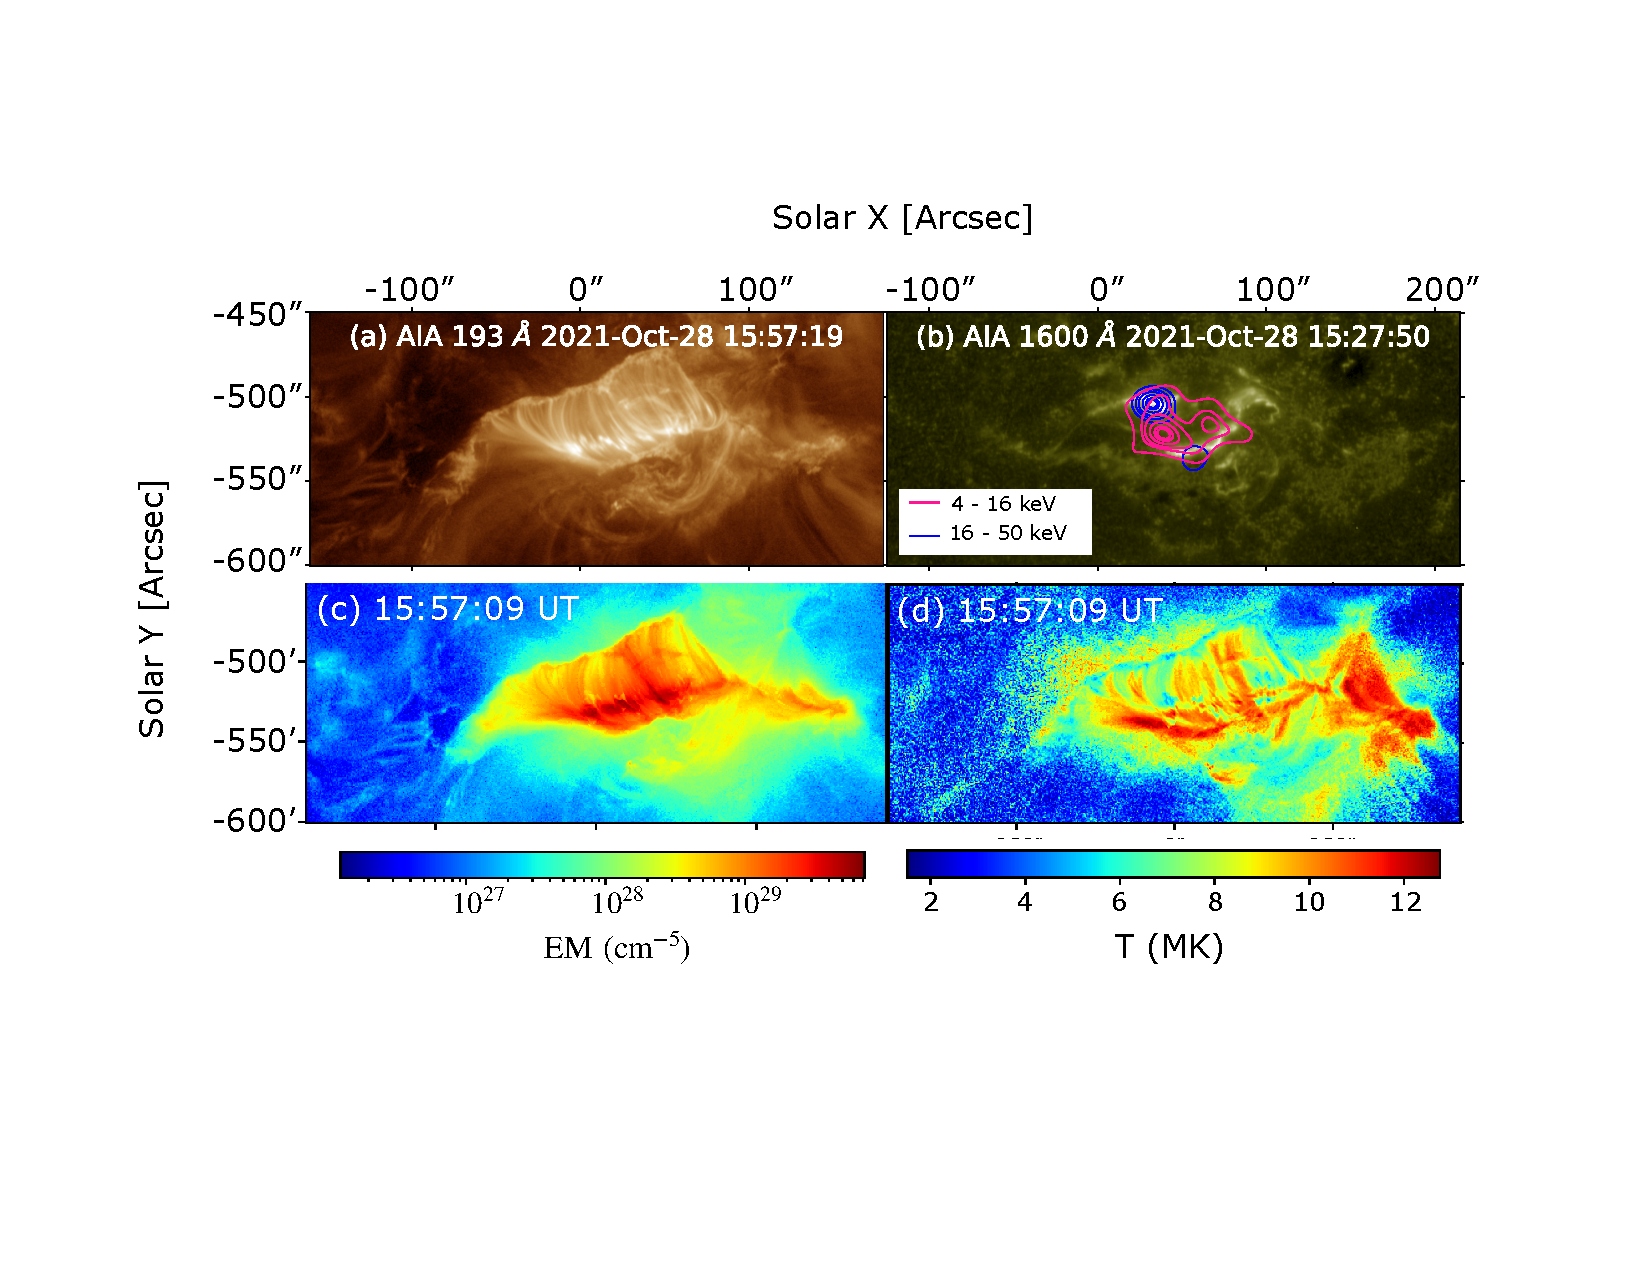
\includegraphics[width=0.9\textwidth,trim={2cm 5cm 3cm 3cm},clip]{oct28_align.pdf}
    \caption{Panel (a): the flare arcade in AIA 193 {\AA}. Panel (b): STIX soft X-ray contours (4 {--} 16 keV, solid pink lines) and hard X-ray contours (16 {--} 50 keV, solid blue lines) aligned to AIA 1600 {\AA} and over plotted. Panel (c): the emission measure map of the region for $5~<log(T)~<7.4$. Panel (d): the DEM weighted temperature map of the region.}
    \label{fig:flare}
\end{figure*}
%%--------------------------

%%--------------------------
\begin{figure*}[ht!]
\centering
    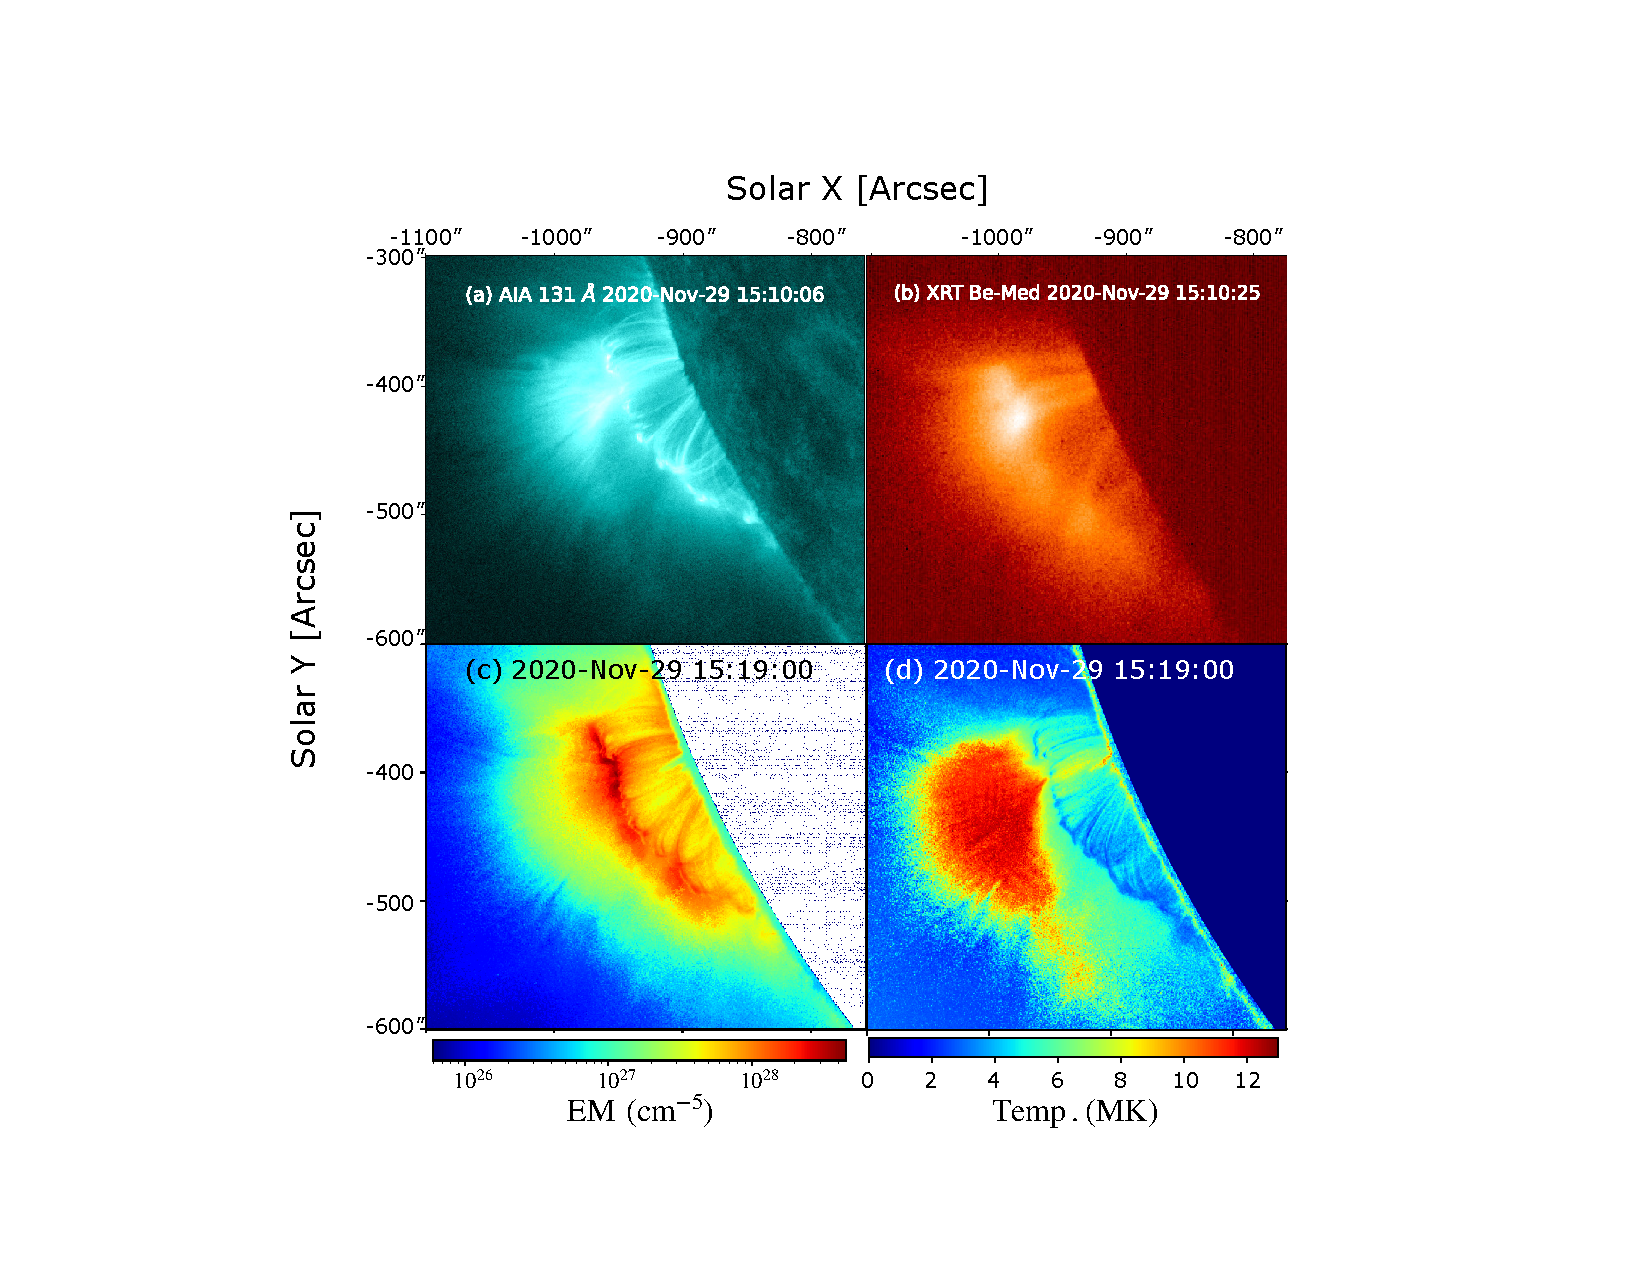
\includegraphics[trim={4.8cm 1.5cm 6cm 2.5cm},clip,width=0.9\textwidth]{nov_29_align.pdf}
    \caption{Panel (a): the flare arcade in AIA 131 {\AA}. Panel (b): {\it Hinode}/XRT Be-Med soft X-ray image recorded almost at the same time. Panel (c):  the DEM weighted temperature map of the region for $5~<log(T)~<7.4$. Panel (d): the emission measure map of the region for $5~<log(T)~<7.4$}
    \label{fig:flare2}
\end{figure*}
%%--------------------------

%%%%%%%%%%%%%%%%%%%%%%%%%%%%%%%%%%%%%%%%
\subsubsection{Determining the LOS}\label{sec:los}
%%%%%%%%%%%%%%%%%%%%%%%%%%%%%%%%%%%%%%%%

To determine the line of sight (LOS) along individual pixels in the field of view (FOV), we initially estimate the height of the flare loop using observations from different vantage points. STEREO-A/EUVI observed both events from a different angle compared to AIA, resulting in geometric effects on the observations.

Fig.\ref{fig:flare_orient}a & b illustrates the geometric effect of observing from different vantage points. The magenta cross in Fig.\ref{fig:flare_orient}a represents a point at the top of the flare arcade. The LOS extends into the page through that point from the STEREO-A vantage. The red line in Fig.\ref{fig:flare_orient}b shows the LOS through the point in Fig.\ref{fig:flare_orient}a projected to the SDO/AIA point of view. Similar projections are shown in Fig.~\ref{fig:flare_orient2} for the Nov 29, 2020 flare.

To calculate the height of the flare loop, we utilize co-temporal STEREO-A 171 {\AA}, 195 {\AA}, and AIA 171 {\AA}, 193 {\AA} images with \textit{scc\_measure.pro}, available in the \textit{sswidl}. This routine enables us to select a point on the observation from one vantage point, and the LOS through the same point is shown on the observation from the other vantage point. By identifying similar emission characteristics, we can determine the 3D coordinates of the point (heliographic latitude, longitude, and radial distance). This measurement is repeated at various positions along the loop top to calculate the change in loop height across the arcade. However, it is important to note that the height estimation using \textit{scc\_measure.pro} is limited by our ability to identify ``similar emission characteristics'' between the AIA and STEREO-A observations.

%%--------------
\begin{figure*}[ht!]
    \centering
    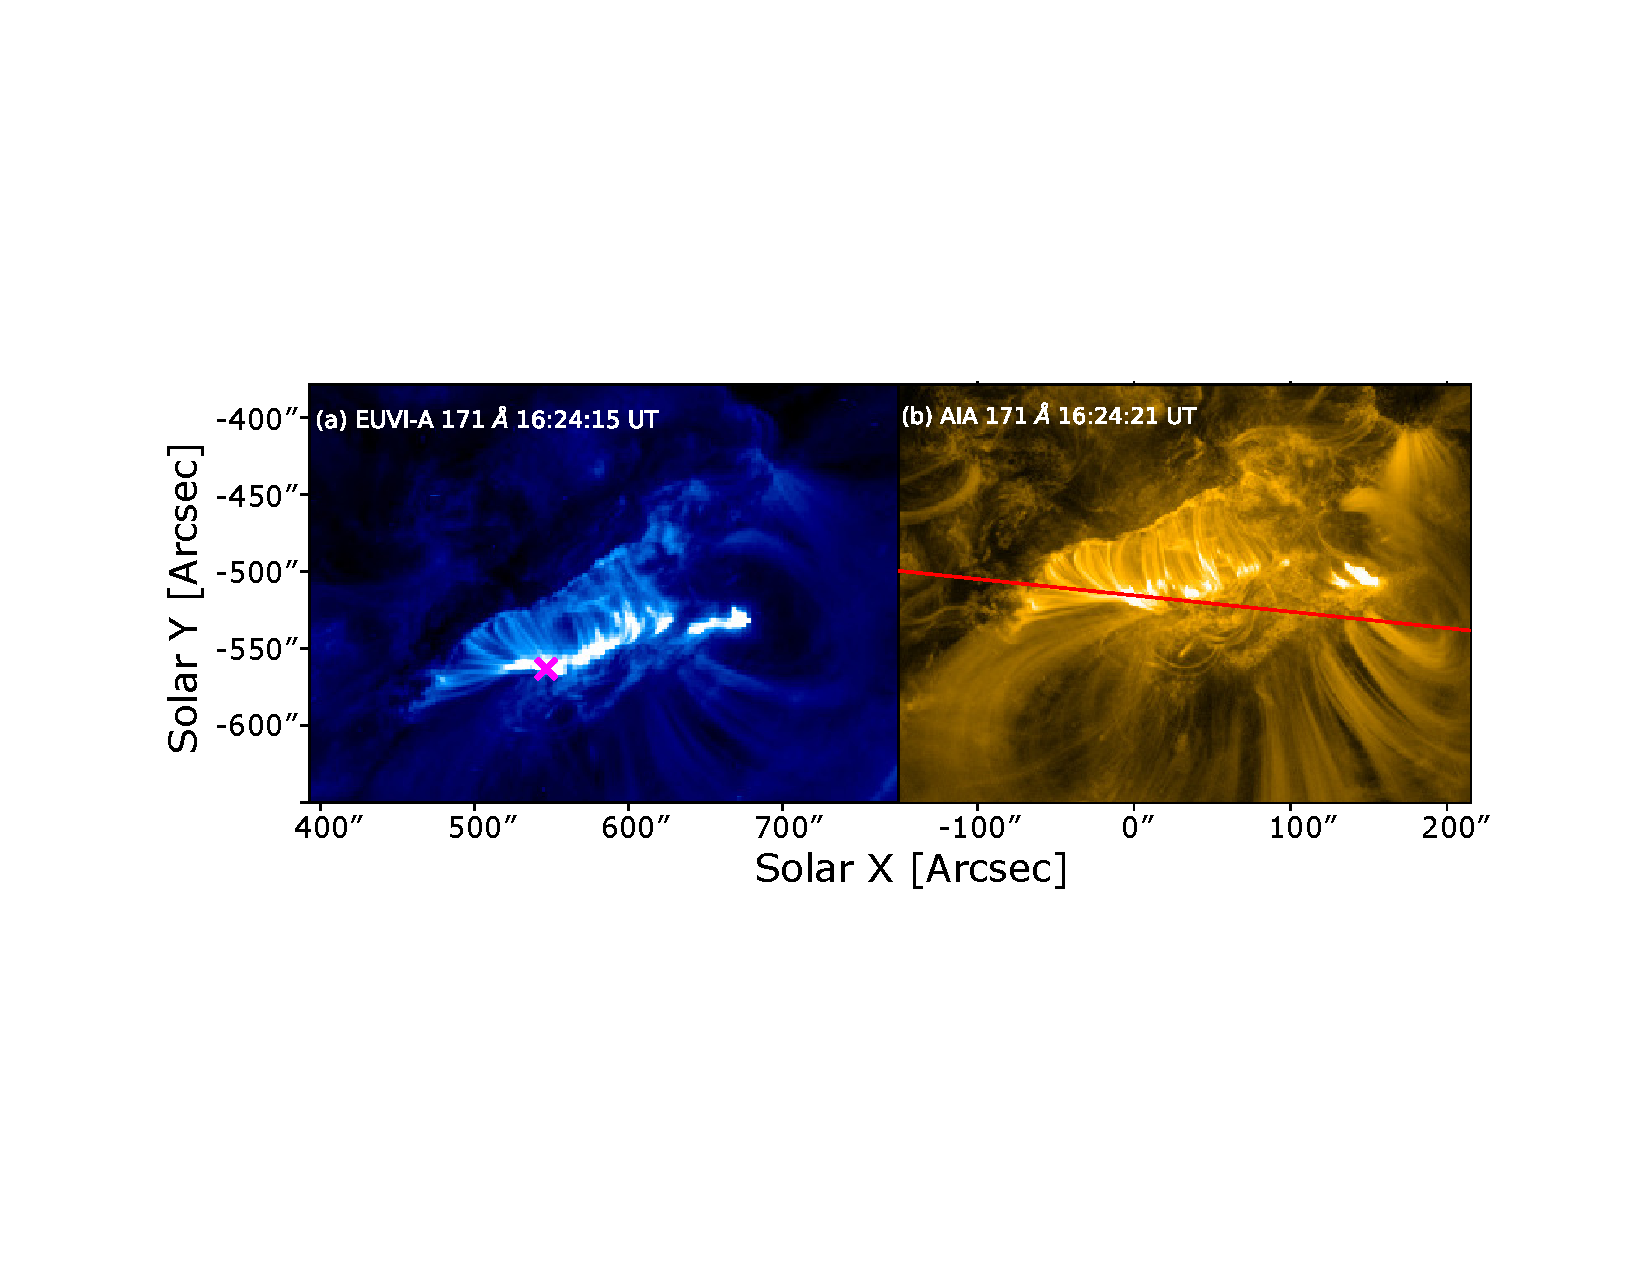
\includegraphics[width=\textwidth,trim={2cm 6cm 2cm 6cm},clip]{flare_orient.pdf}
    \caption{Panel (a): {\it STEREO-A}/EUVI 171 {\AA} observation of the flare arcade in the decay phase. The magenta cross marks a point on the top of the arcade. The LOS goes into the page through that point. Panel (b): SDO/AIA 171 {\AA} observation of the flare arcade. The red line marks the LOS through the arcade from the STEREO-A perspective projected to the AIA perspective.}
    \label{fig:flare_orient}
\end{figure*}
%%--------------

%%--------------
\begin{figure*}[ht!]
    \centering
    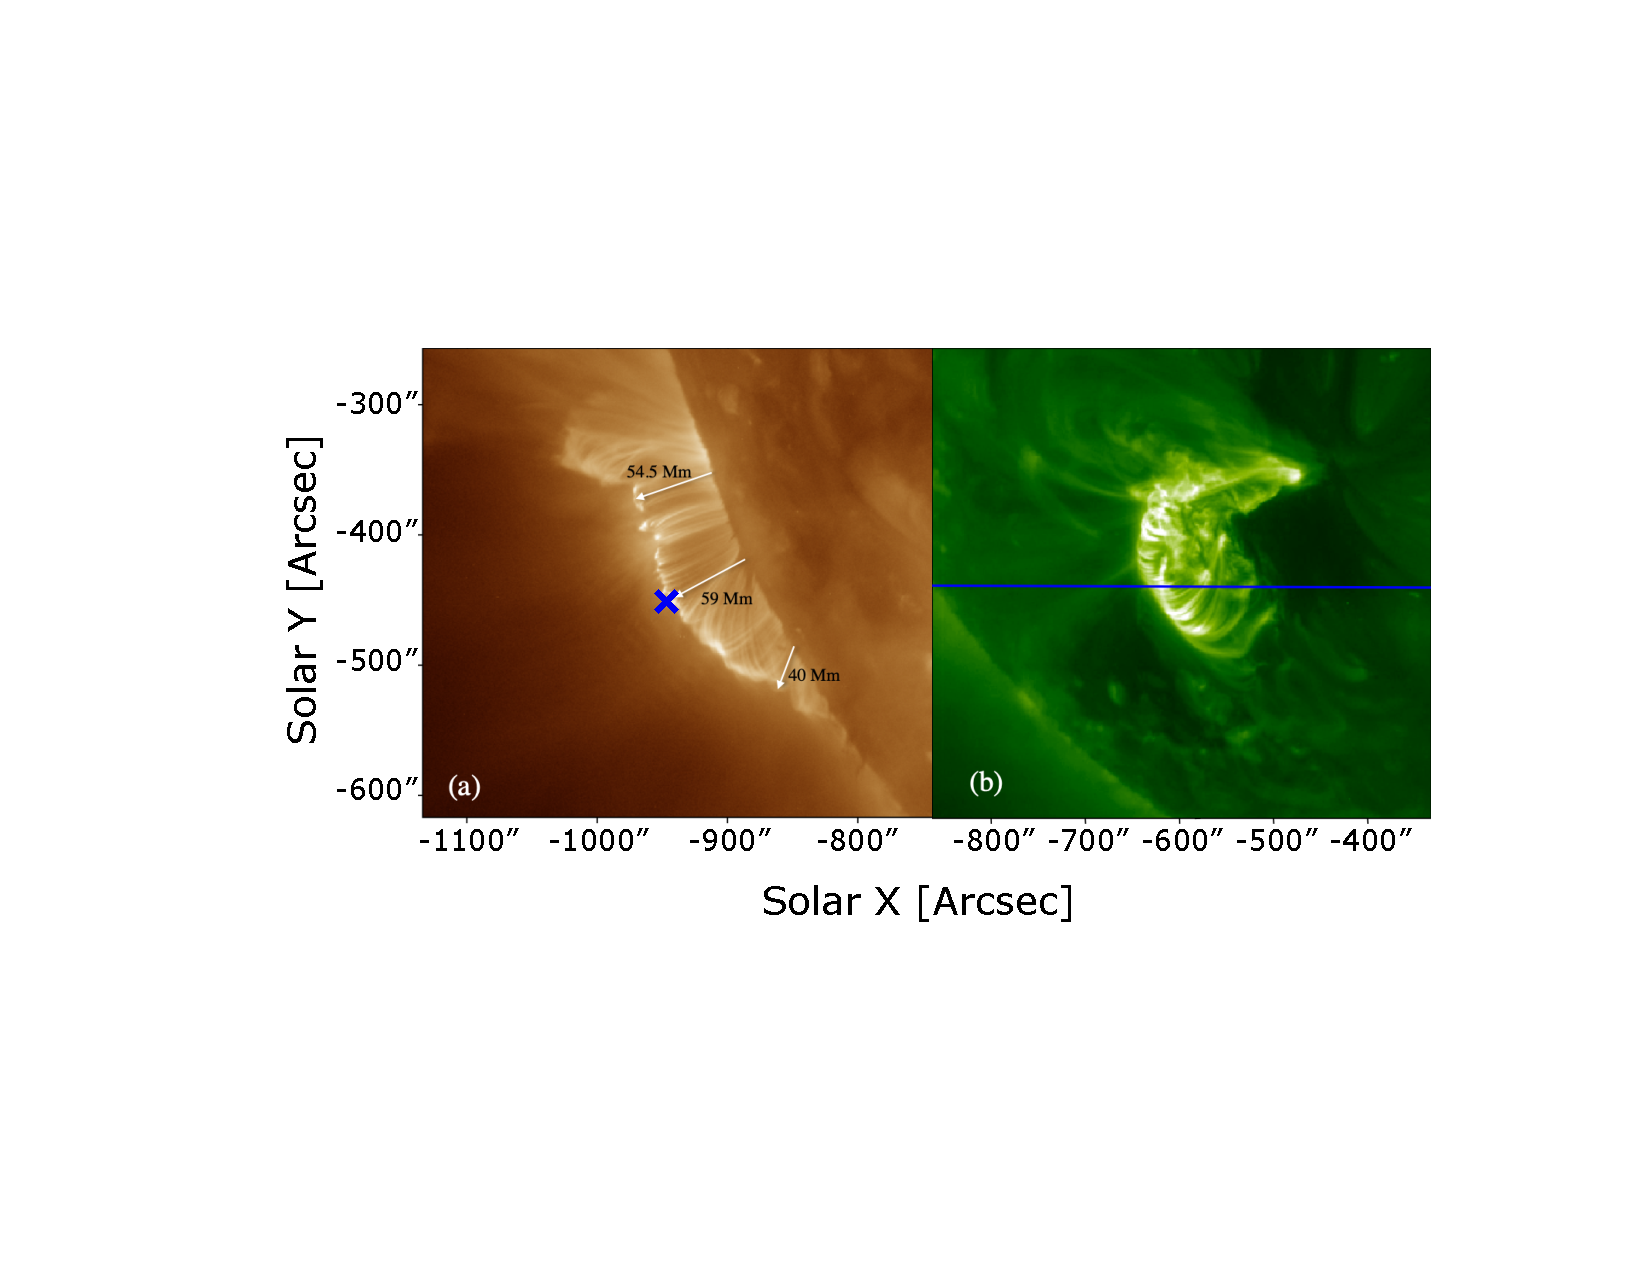
\includegraphics[width=0.9\textwidth,trim={4cm 5cm 3cm 5cm},clip]{nov29_triangulate.pdf}
    \caption{Panel (a): SDO/AIA 193 {\AA} observation of the Nov 29 flare in the decay phase. The blue cross marks a point on the top of the arcade. The LOS goes into the page from AIA perspective. Panel (b): {\it STEREO-A}/EUVI 195 {\AA} observation around same time. The blue solid line is the LOS from AIA perspective in panel (a) projected onto {\it STEREO-A} perspective. We can trace out the height of the flare arcade at various locations using \textit{scc\_measure.pro}. The height of the arcade at various points from the Sun's surface is marked in panel (a).}
    \label{fig:flare_orient2}
    \end{figure*}
%%--------------

%%--------------
\begin{figure*}[ht!]
    \centering
    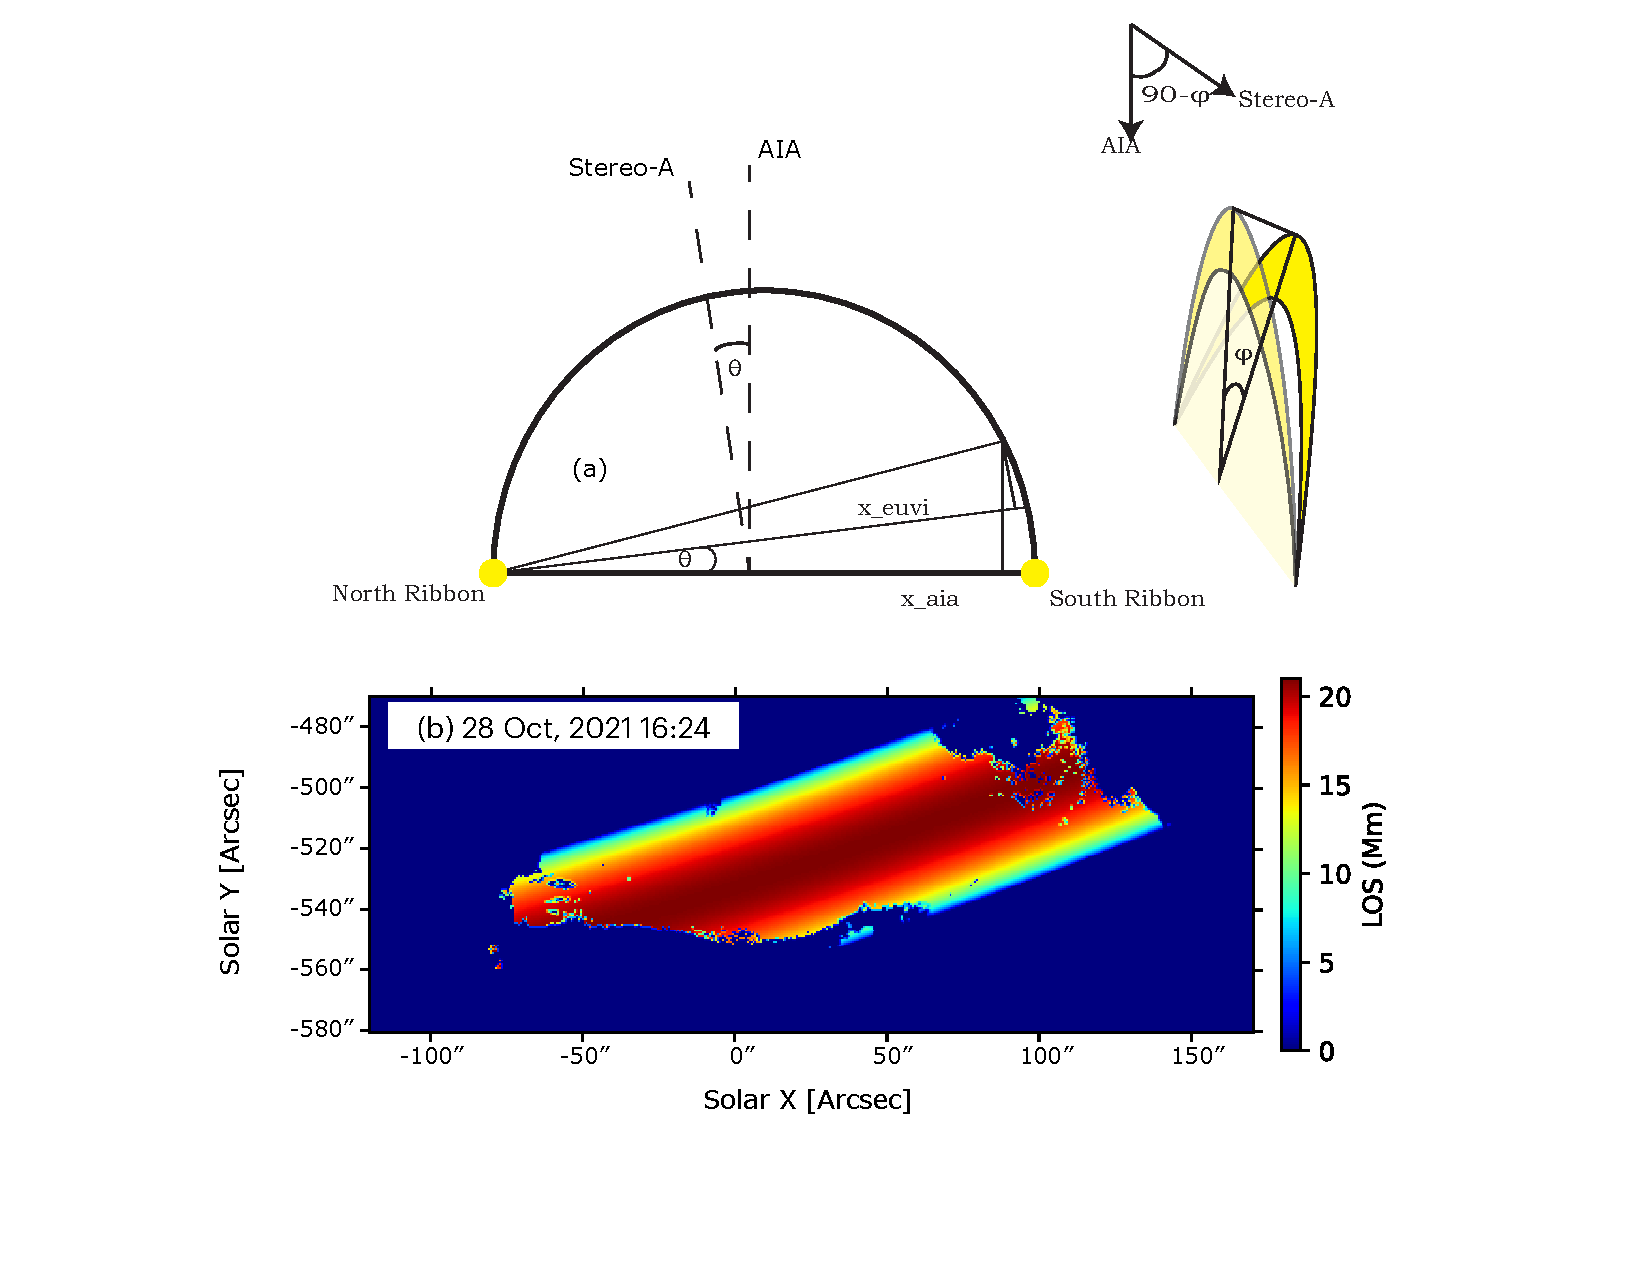
\includegraphics[width=0.8\textwidth,trim={3cm 2cm 3cm 0cm},clip]{flare_orient_pt2.pdf}
    \caption{Panel (a): Cartoon demonstrating the projection effects of a semicircular loop between STEREO-A and AIA vantages due to the difference between polar ($\theta$) and azimuthal ($\phi$) angles, respectively. Panel (b) : The calculated LOS map from the AIA perspective, with the estimated loop top height under the assumption of a semi-circular loop geometry.}
    \label{fig:flare_orient_2}
\end{figure*}
%%--------------

To determine the extent of the flare arcade, we select pixels within an emission measure contour of 5\% of the peak emission measure value. This contour is calculated based on the emission measure inferred from the DEM, which reflects the density of plasma across the temperature range of $5<\log,(T)<7.4$. This approach provides a more comprehensive estimate of the flare arcade compared to methods based solely on intensity observations, which may miss significant portions of the arcade due to the highly multi-thermal nature of the plasma. Outside of the flare arcade, we assume a line of sight (LOS) thickness of approximately 2 Mm, corresponding to the average thickness of the chromosphere.

Fig. \ref{fig:flare_orient_2}b illustrates an example of the calculated LOS in the field of view (FOV) for the October 28, 2021 flare. The highest point of the flare arcade follows the ridge from southeast to northwest. An estimate of the highest point of the loop is approximately 22 Mm, consistent with previous estimates of the ridge height around 20 Mm from magnetic loop modeling \citep{longcope22}. Using the LOS map shown in the bottom panel of Fig. \ref{fig:flare_orient_2}, we calculate the thermal energy in every pixel of the flare using Equation \ref{eq:t_eneg}. This process is repeated for the flare loops in the November 29, 2020 event.

%%%%%%%%%%%%%%%%%%%%%%%%%%%%%%%%%%%%%%%%%%%%%%%%%%%%
\subsection{Energy in the non-thermal electrons}\label{sec:non-therm}
%%%%%%%%%%%%%%%%%%%%%%%%%%%%%%%%%%%%%%%%%%%%%%%%%%%%

To estimate the energy deposited by the non-thermal electrons in the X-class event on October 28, 2021, we analyze the STIX spectra. Figure \ref{fig:stix_an}.a illustrates the STIX light curve for different energy bands: 4 to 6 keV (solid black line), 6 to 12 keV (solid magenta line), 12 to 25 keV (solid yellow line), and 25 to 50 keV (solid blue line). The attenuator was activated around 15:28 UT to prevent saturation, notably reducing the intensity. The hard X-ray peak appears around 25 to 50 keV at approximately 15:28 UT, while the soft X-ray peak is discernible within the attenuated flux in the 6 to 12 keV band at approximately 15:30 UT.

Following the methodology outlined in \cite{emslie12}, we fit the STIX spectra at various time intervals during the flare's evolution using the `2vth' and `thick2' functions available in the OSPEX X-ray spectra fitting package within `{\it sswidl}'. A representative fit is depicted in Figure \ref{fig:stix_an} panel (b) for the time bin around 15:26-15:27 UT using the `2vth' (solid yellow) and `thick2' (solid green) functions. The `2vth' function represents a two-component thermal model, with parameters for emission measure, temperature of the thermal components, and relative abundances of various elements with respect to CHIANTI coronal abundances \citep{chianti1,chianti}. On the other hand, the `thick2' function assumes a non-thermal component attributed to bremsstrahlung from energetic electrons, described by a broken power-law injected spectrum $F_{0}(E_{0})~(e^{-}s^{-1}cm^{-2}keV^{-1})$ :

%%--------
\begin{equation}
    F_{0}(E_{0})=A
    \begin{cases}
        0, & E_{0}<E_{min} \\
        E_{0}^{-\delta_{1}}, & E_{min} \le E_{0} < E_{b} \\
        E_{0}^{-\delta_{2}}E_{b}^{\delta_{2}-\delta_{1}}, & E_{b} \le E_{0} < E_{max} \\
        0, & E_{max} \le E_{0}
    \end{cases}
\end{equation}
%%--------

In the fitting process, the model spectrum parameters, such as the normalization parameter \( A \), the low- and high-energy cutoffs \( E_{\text{min}} \) and \( E_{\text{max}} \), the break energy \( E_{\text{b}} \), and the power law indices \( \delta_{1} \) and \( \delta_{2} \) below and above the break, are constrained. We set the high-energy cutoff at \( 3.2 \times 10^{4} \) keV for all fits, as it is significantly higher than the energy range of interest (around \( 10^{1} \) keV), making its effect on the X-ray spectra negligible \citep{emslie12}.

The fitting procedure in `\textit{OSPEX}' is a forward fitting process. The parameters of the `\textit{2vth}' and `\textit{thick2}' functions are adjusted to generate a photon spectrum, which is then convolved through the detector response matrix to produce a count rate spectrum. This count rate spectrum is compared with the measured count rate spectrum, and an iterative process minimizes the \( \chi^{2} \) between them to refine the parameter estimates.

Table \ref{tab1} presents the fitted temperature of the hotter thermal component at various phases of the flare. These temperatures align with the temperature range (\( \log(T_{\text{max}}) = 7.4 \) and \( \log(T_{\text{min}}) = 5 \)) used to calculate the emission measure (EM) and differential emission measure (DEM) weighted temperature, as discussed in Section \ref{sec:therm}.

%%%%%%%%%%%
\begin{table*}[ht!]
    \centering
    \begin{tabular}{|cl||c|c|}
    \hline
         &  & log(T) & EM \\ 
         & \hspace{-1cm}Time (UT) & of hotter component & ($cm^{-3}$) \\
    \hline
        Impulsive phase & \hspace{1cm}15:26 & 7.098 & $10^{48}$\\
        HXR peak & $\sim$ 15:27:20 - 15:28:20 & 7.19 & $3\times 10^{48}$\\
        Right after SXR peak & $\sim$ 15:35:39 - 15:36:34 & 6.88 & $4.1\times 10^{49}$\\
        Into the decay phase & \hspace{0.9cm}14:48:20 & 6.5 & $2\times 10^{49}$\\
        \hline
    \end{tabular}
    \caption{Fitted temperature of the hotter component of the thermal plasma during various stages of the flare.}
    \label{tab1}
\end{table*}
%%%%%%%%%%%

The non-thermal energy in the electrons (\( U_{e} \)) at any instant \( t = t' \) can be estimated by integrating the best-fit electron energy spectrum:
\[
U_{e}(t=t') = \Delta t \int_{E_{\text{min}}}^{E_{\text{max}}} F_{0}(E_{0})(t=t') dE_{0}
\]
where the electron energy distribution is constrained by fitting the count spectra for the time interval \( t' - \Delta t/2 \leq t \leq t' + \Delta t/2 \).

The cumulative energy deposited into the footpoint over time by the non-thermal electrons is a good indicator of the source of the thermal energy of the plasma. We can estimate the cumulative energy deposited by the non-thermal electrons up until a certain instant \( t \) by summing the energy deposited at the footpoints from every time bin:
\[
U^{cumulative}_{e}(t) = \sum_{t'=t_{0}}^{t} U_{e}(t')
\]

%%--------------
\begin{figure*}[ht!]
    \centering
    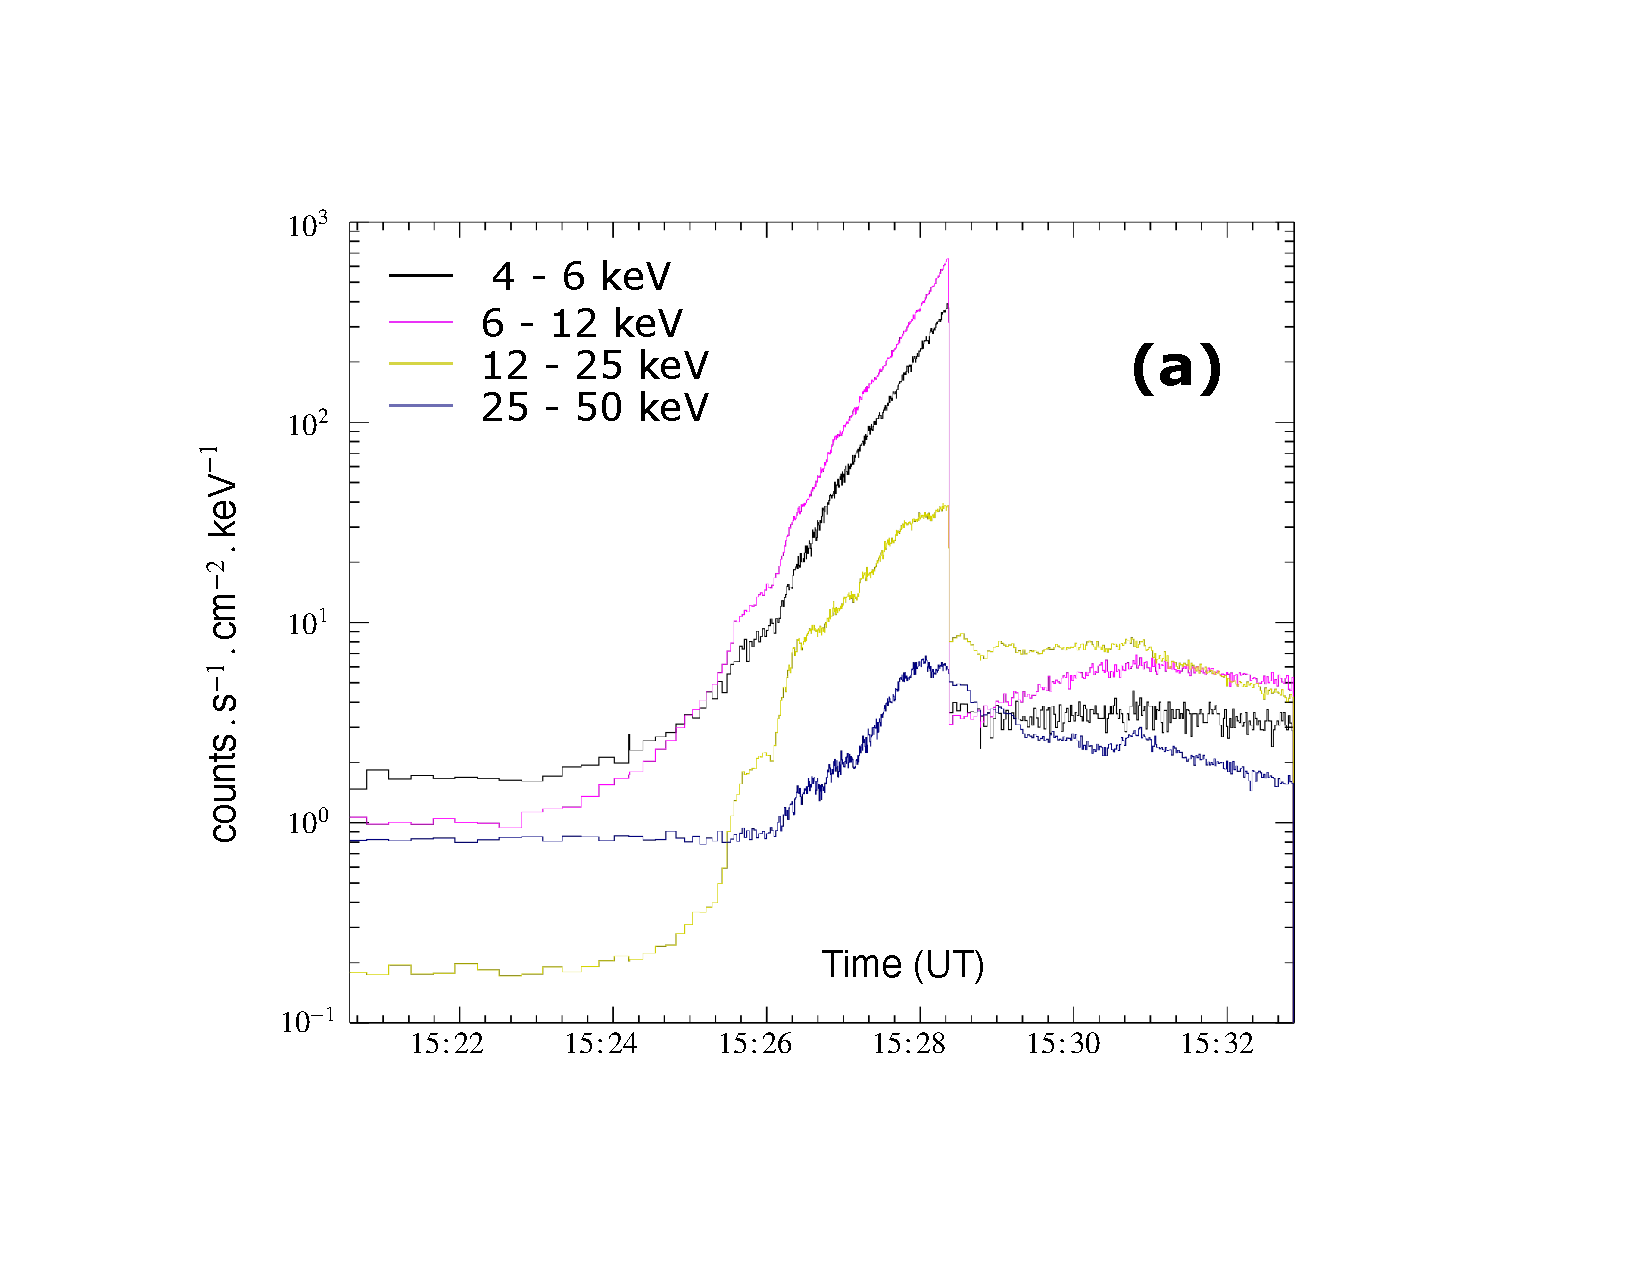
\includegraphics[trim={3cm 2cm 6cm 3.5cm},clip,width=0.54\textwidth]{oct28_lc_2.pdf} 
    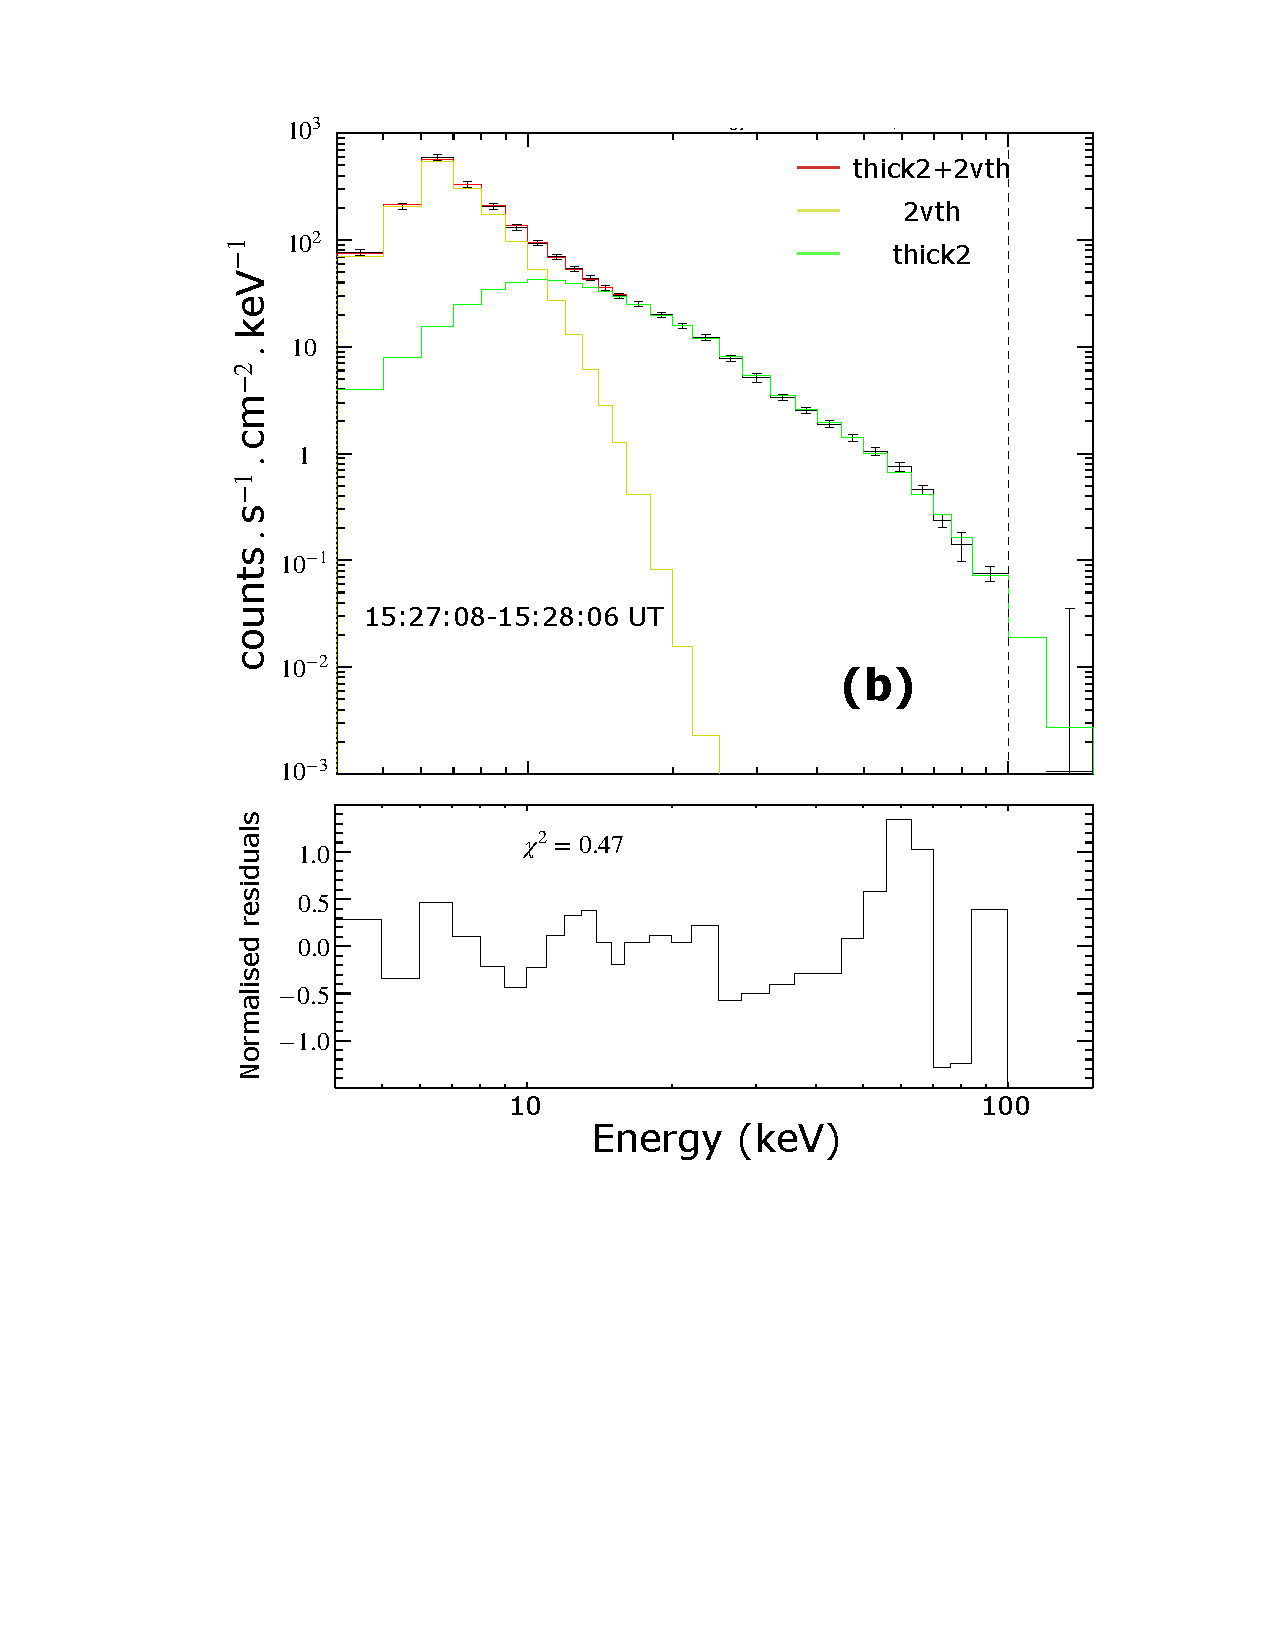
\includegraphics[trim={3.5cm 8cm 3cm 2cm},clip,width=0.45\textwidth]{oct28_fit_2.pdf}
    \caption{Panel (a): STIX light curve of the 2021 Oct 28 X-class event in different energy bands as labelled. The black, magenta, yellow and blue solid lines show the light curve in 4{--}6~keV, 6{--}12~keV, 12{--}25~keV and 25{--}50 keV. Panel (b): STIX spectra fit at 15:27{--}15:28 UT, during impulsive phase. We fit the spectra with `\textit{thcik2}' (green solid line) and `\textit{2vth}' (yellow solid line). We show the complete fit function `\textit{2vth+thick2}' with the solid red line. The lower panel shows the normalized residuals of the fit.}
    \label{fig:stix_an}
    \end{figure*}
%%--------------

%%%%%%%%%%%%%%%%%%%%%%%%%%%%%%%%%%%%%%%%%%%%%
\section{Results}\label{res}
%%%%%%%%%%%%%%%%%%%%%%%%%%%%%%%%%%%%%%%%%%%%%

%%###########%%
\begin{figure}[ht!]
    \centering
    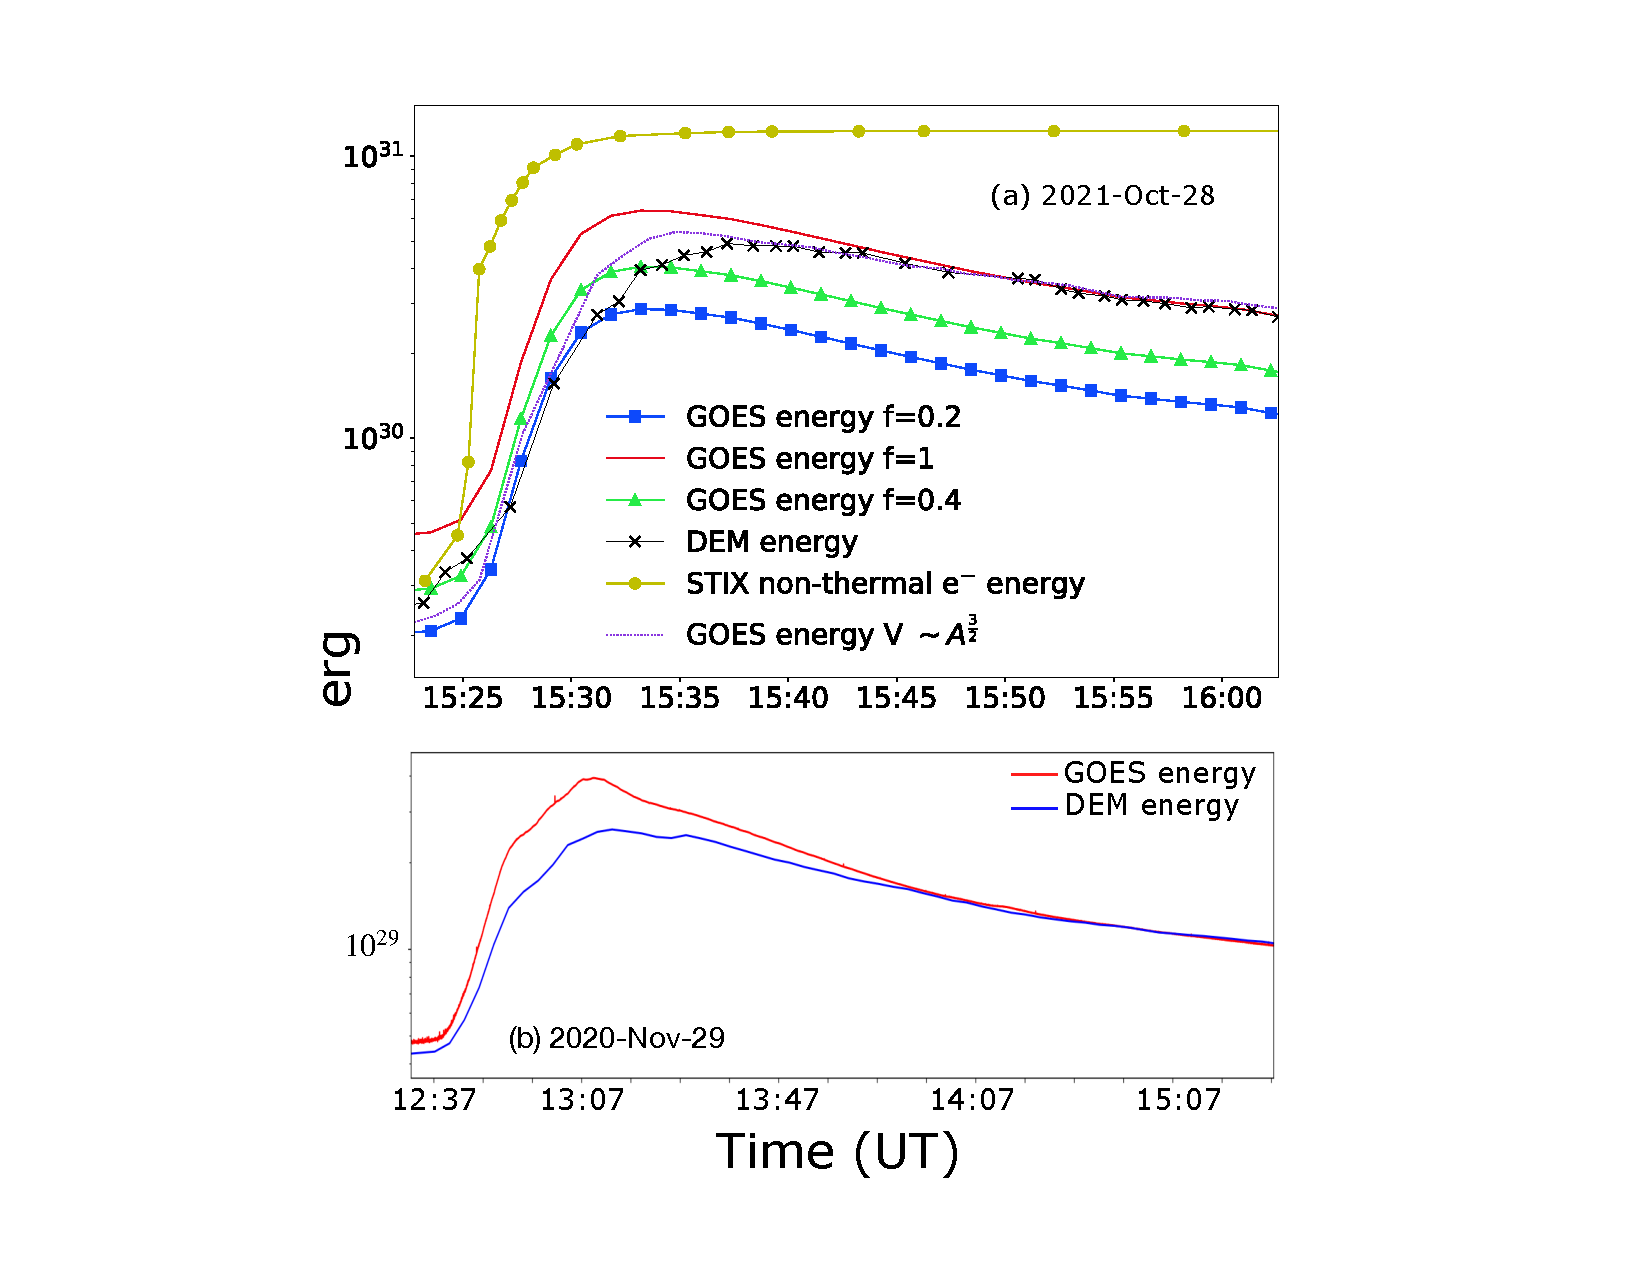
\includegraphics[trim={4cm 1cm 4cm 1cm},clip,width=0.8\textwidth]{flare_eneg.pdf}
    \caption{Panel (a): The calculated thermal energy as a function of time for the 2021 Oct 28 flare. The magenta dot-dashed line shows the thermal energy calculated from the GOES light-curve using the effective volume and a filling factor \textit{f}~=~1. The red dot-dashed line and the black dashed line shows the energy calculated from the GOES light-curve and the effective volume with filling factor \textit{f}~=~0.4 and \textit{f}~=~0.2, respectively. The blue solid line shows the thermal energy estimated using the DEMs calculated from the AIA obeservations. The black solid line shows the thermal energy calculated from the GOES light curve, but the volume inferred from the area of the of the flaring arcade with STIX SXR images, under the assumption that $V\sim A^{\frac{3}{2}}$. Panel (b): The calculated thermal energy as a function of time for the 2020 Nov 29 flare. The red line shows the thermal energy calculated from the GOES light curves, using a constant effective volume. The blue curve shows the thermal energy calculated from the DEMs inferred from the imaging and a varying volume from the imaging.}
    \label{fig:eneg}
\end{figure}
%%###########%%

%%###########%%
\begin{figure}[ht!]
    \centering
    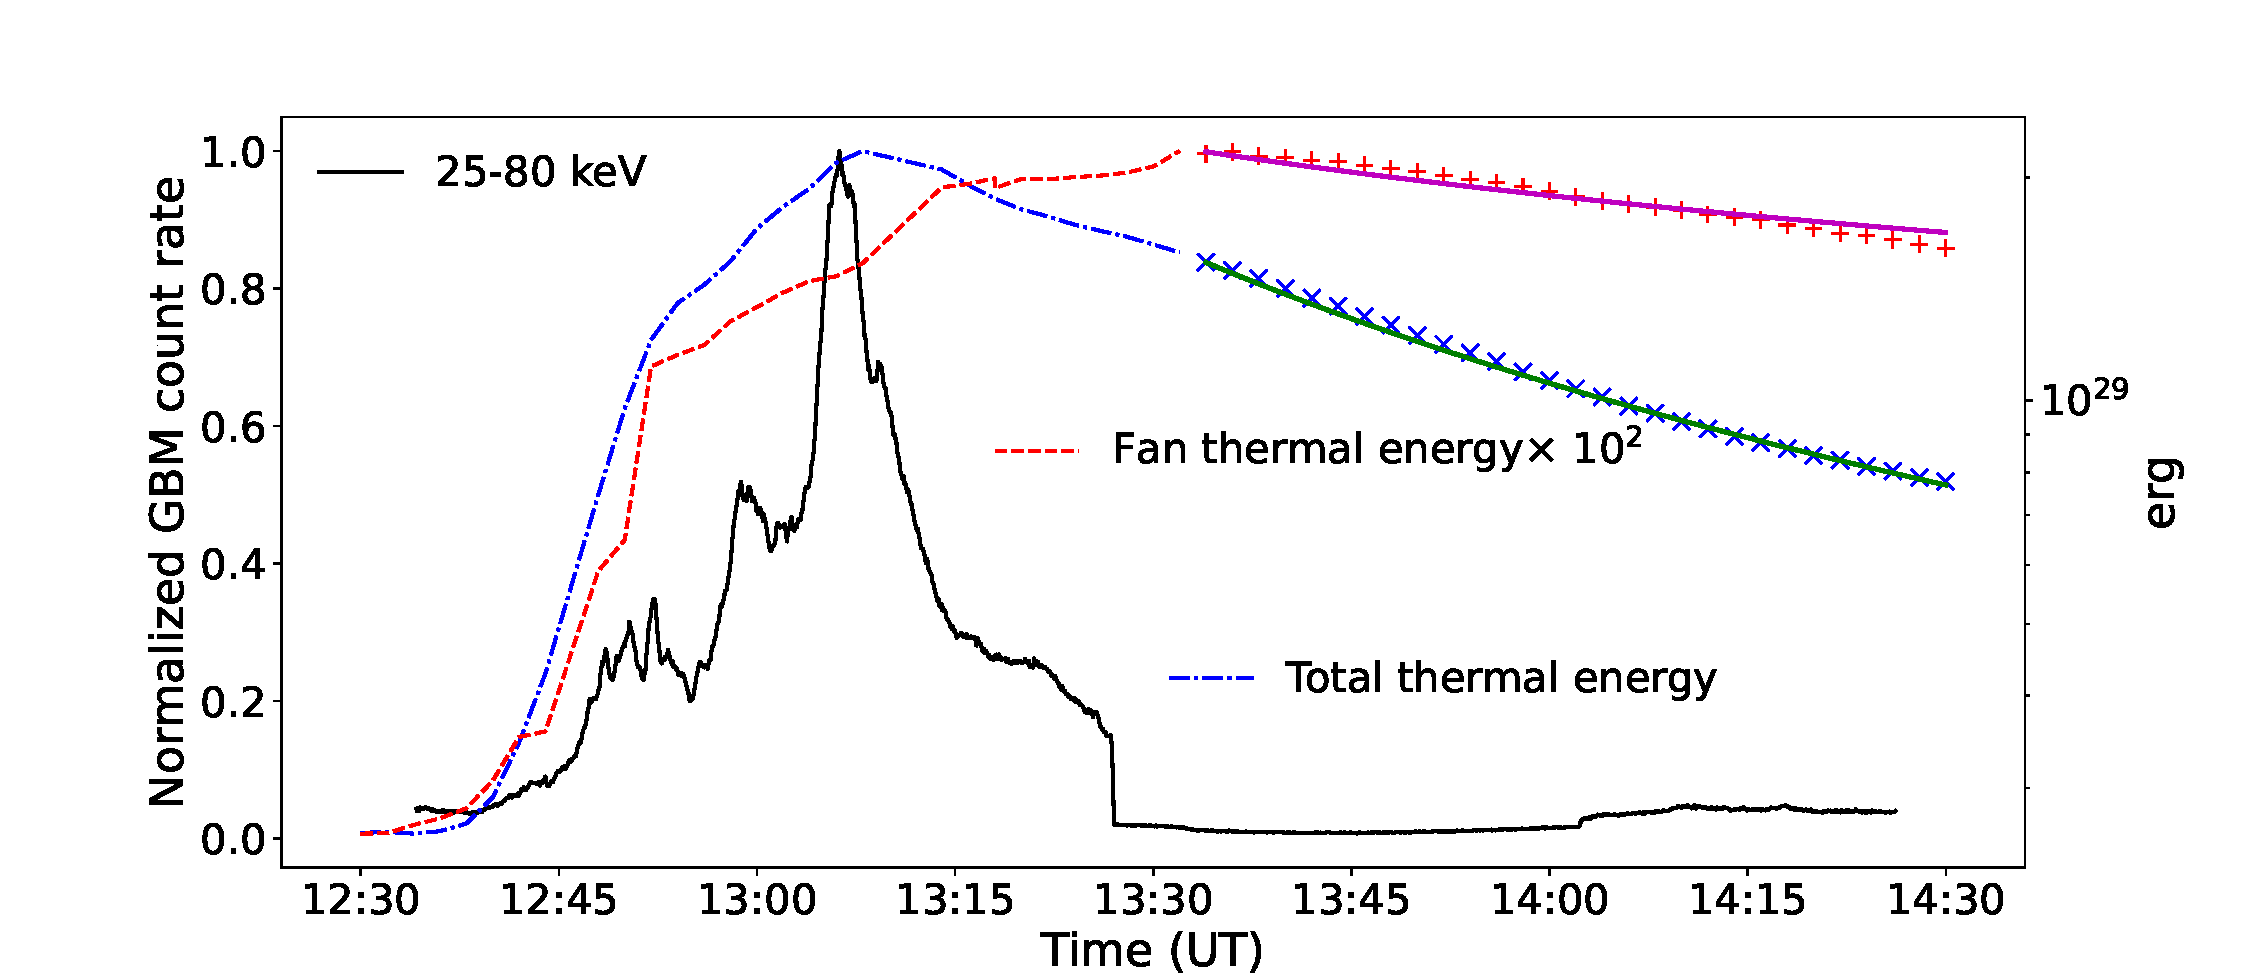
\includegraphics[trim={2cm 0cm 1cm 0cm},clip,width=0.8\textwidth]{fan_eneg.pdf}
    \caption{Calculated thermal energy for the 2020 Nov 29 flare. Total thermal energy of the flare (blue dot-dashed) in comparison to the thermal energy from the fan (red dashed). The magenta and the green solid line show the fit to the thermal energy output to the fan and the loop's thermal output. Fermi hard X-ray count (black) peaks around the same time as the total thermal output.}
    \label{fig:fan_eneg}
    \end{figure}
%%###########%% 

Figure~\ref{fig:eneg}.a shows the thermal and non-thermal energy calculated for the 2021 October 28 event. The black solid curve with crosses shows the thermal energy calculated from the DEMs. The red solid curve shows the thermal energy calculated from the {\it GOES} light curve and the effective volume calculated assuming an RTV loop \citep{rtv78,serio91}. We use the {\it GOES} emission measure, temperature with a volume filling factor \textit{f}~=~1, to estimate an effective loop length for the flare and from that, calculate an effective volume. Note that the implicit assumption of mechanical equilibrium only holds during the decay phase of the flare. So, the effective volume estimated here would only be appropriate in the decay phase. The green solid curve with triangles and the blue solid curve with squares show the same {\it GOES} thermal energy, with volume filling factor \textit{f}~=~0.4 and \textit{f}~=~0.2, respectively. The blue dashed curve shows the thermal energy calculated from the {\it GOES} light curve, but the volume inferred from the area of the flaring region from the STIX soft X-ray contours, under the assumption that $V\sim A^{\frac{3}{2}}$.

The lime green solid line with circles in Fig.~\ref{fig:eneg}.a, shows the cumulative energy in the non-thermal electrons. This quantity is the amount of energy deposited at the flare foot points, and one of the sources of the thermal energy of the flare. The cumulative non-thermal energy of electrons $\simeq~1.2\times 10^{31}$ erg $>$ peak thermal energy calculated from the DEM estimates $\simeq~5\times 10^{30}$ erg. This is usual for an X-class flare. The differences in the estimates of thermal energy, due to different estimations of volume, also affects the partition between the thermal and non-thermal energies of flares. The efficiency of converting the energy deposited by non-thermal electrons into the thermal energy of the ambient plasma results in this partition and as a result, the volume estimation is a key parameter in understanding the conversion of non-thermal energy into thermal energy in flares.

The interesting trend in Fig.~\ref{fig:eneg}.a is that the thermal energy calculated from the constrained DEMs (solid black curve with crosses) is closer to a volume filling factor \textit{f}~=~0.2 in the impulsive phase, but is asymptotic with a filling factor \textit{f}~=~1 (solid red curve) during the decay phase. This indicates that the flare loops during the impulsive phase do not fill up apparent volumes similar to those in the decay phase. The change in the effective filling factor is indicative of the sharp change in the volume during the impulsive phase.

For the 2020 November 29 event, the {\it STEREO-A} perspective looks down into the supra-arcade plasma sheet. Thus the LOS of this feature can not be calculated as demonstrated in Section \ref{sec:los} for the supra-arcade pixels. For the supra-arcade fan pixels in the FOV, we assume a LOS $\simeq~8~\textrm{Mm}$, as suggested in several other studies \citep[see e.g.,][]{savage10,seaton17,li18}. We use these calculated LOS maps, along with equation~\ref{eq:t_eneg_1} to estimate the thermal energy as a function of time.

Figure \ref{fig:eneg}.b shows the energy calculated for the November 29th event. The blue solid curve shows the thermal energy calculated from the DEMs. The red solid curve shows the thermal energy calculated from the GOES light curves and the constant effective volume calculated assuming an RTV loop with a volume filling factor \textit{f}~=~1. The thermal energy shows similar characteristics as the October 28th, 2021 event. The RTV loop effective volume clearly is an overestimation in the rise phase of the the flare, and agrees very well in the decay phase.

There have been several studies that suggest that the plasma in the fan is directly heated \citep{hanneman14,chen17,reeves17,warren18,cai22,xie23}. Unlike the flare arcade, the thermal output of the fan is not directly related to the energy deposited by the non-thermal electrons and ions at the foot point. Hence, this different mechanism should also be reflected in the time evolution of the thermal output of the fan, compared to the thermal output of the loops. Under the assumption of the LOS~$\mathrm{\sim 8~Mm}$ in the fan region, we separately calculate the contribution from the fan to the total thermal energy for the 2020 Nov 29 event.

Figure~\ref{fig:fan_eneg} shows the thermal energy of the fan as a function of time (red dashed line) in comparison to the total thermal energy of the 2020 Nov 29 event (blue dot-dashed line). The thermal energy form the fan is $\sim$ two orders of magnitude lower than the total thermal energy of the event. The thermal energy of the fan also peaks much later ($\sim$ 20 minutes) compared to the total thermal energy. After the thermal energy of the fan peaks, the thermal energy of the fan (red + sign) and the total thermal energy of the event (blue crosses) are fitted with a power law of the form $at^{-\delta}$ as a function of time. The fits are shown with magenta and green solid line for the fan and the total thermal energy, respectively. The value of the power law index are -0.95 and -1.1, respectively, for the fan and the total thermal output. The plots shows that the thermal energy of the fan decay slower compared to the total thermal output. The normalized {\it Fermi} GBM 25 {--} 80 keV count rate (black solid line) peaks at a similar time as the total thermal energy of the event.

%%%%%%%%%%%%%%%%%%%%%%%%%%%%%%%%%%%%%%%%%%%%%
\section{Outlook}\label{sec:out}
%%%%%%%%%%%%%%%%%%%%%%%%%%%%%%%%%%%%%%%%%%%%% 


We have used AIA, SUVI, and XRT observations to calculate DEM maps and estimate the thermal energy for two solar flares as a function of time. We have used observations from AIA and {\it STEREO-A} to calculate the geometry of the flare loops and estimate the LOS for the AIA observations. We have shown that the accurate estimation of volume can have significant implications for thermal energy estimates. For the 2020 November 20 flare, we have also estimated the thermal energy for the fan and compared the evolution of the thermal energy of the fan with respect to the total thermal energy of the event. We have shown that the thermal energy of the fan decays slower compared to the total thermal energy of the event. This result suggests that a fundamentally different heating mechanism is responsible for the thermal output of the fan.

The thermal energy of the flares is given as, $U_{Th}\simeq 3n_{e}k_{B}TVf$. The electron number density is given by, $n_{e}~=~\sqrt{\sfrac{EM^{v}}{Vf}}~\implies~U_{Th}~=~3k_{B}T\sqrt{EM^{v}\times~Vf}$, where $EM^{v}$ is the volume emission measure (in units of $cm^{-3}$). A filling factor, \textit{f} $<$ 1 decreases the thermal energy by $\sim f^{\sfrac{1}{2}}$. There are very diverse results reported on \textit{f}. X-ray observations have generally constrained within $0.1<\textit{f}<1$\citep{jak11,guo12}, while it is usually constrained to much lower values $0.001<\textit{f}<0.1$ in EUV\citep{ash&ash08}. The filling factor can also be constrained by imposing the requirement that the flare plasma has to be contained via magnetic pressure. From this constraint it can be inferred that the required coronal magnetic field strength $B_{cor}$ $\sim f^{-\sfrac{1}{4}}$\citep{caspi14,warmuth16a,warmuth16b}. These studies rule out values of $\textit{f}<0.1$. Similar results were obtained from spectroscopic observations of density sensitive \ion{Fe}{11} lines \citep{miligan12}.

It is easy to infer from our findings that a single value of volume filling factor is inadequate to describe the evolution of thermal energy throughout the duration of the flare. We need to estimate the volume as a function of time rather than depending on a filling factor. In Fig.~\ref{fig:eneg}.a, the thermal energy calculated from {\it GOES} with various filling factors demonstrates this concept perfectly. During the impulsive phase, the thermal energy calculated from the DEMs is consistent with \textit{f}=0.2, and later in the decay phase, it is consistent with \textit{f}=1. This result demonstrates how the volume of the flare arcade is changing over time with respect to the volume in the decay phase. The thermal energy calculated from $V\sim A^{\frac{3}{2}}$ assumption agrees well with the thermal energy calculated from constrained DEMs in the decay phase. But it still predicts higher energy in the impulsive phase. This discrepancy might signify that the assumption of self-similar expansion might not be valid at the initial sharp rise in the impulsive phase for some flares.

Our results are in line with the findings of \cite{hilarie05}. They demonstrated from {\it RHESSI} imaging for a sample of 9 M and C class flares that the volume estimation with the assumption of self-similar expansion resulted in thermal energy higher than the non-thermal energy during the impulsive phase (For more details, refer to \cite{hilarie05} Table 5 and the corresponding discussion). A statistically inferred representative filling factor might serve perfectly well for estimating the energies near the thermal peak for a sample of flares. Since we are trying to quantify the evolution of the energy over time for individual flares, we require more accurate estimates of the volume.

Our results also demonstrate the utility of estimating the volume from different vantages as a function of time. For events like the X-class event on 2021 October 28, the on-disk imaging allows the estimation of the volume from the flare ribbon area under the assumption of self-similar expansion. But for scenarios like the limb event 2020 November 29, where the flare ribbons are not visible from any imaging observation, or the visible foot point and/or visible portions of the loop are projected at a very high angle, estimating the volume of the loop by calculating the height of the loop at various points serves as an important tool in estimating the thermal energy at various phases of the flare.

In Figure~\ref{fig:fan_eneg}, the thermal energy from the fan (red dashed line ) is $\sim$ two orders of magnitude lower than the total thermal energy of the event (blue dot-dashed line). The thermal energy also peaks much later ($\sim$ 20 minutes) compared to the total thermal energy. This result shows that the fan plasma is being heated directly by a process different from the flare arcade (e.g. SADs \citep{reeves17}, plasma flow turbulence \citep{xie23}). The fan also cools slower than the arcade, which indicates that either continuous heating is present in the fan during the decay phase of the flare or there is suppression of cooling \citep[e.g.][]{xie23}. The event had both foot points occulted from the Earth's perspective, so it is a fair assumption that most of the hard X-ray is from the loop top coronal source. This circumstance explains the near-simultaneous peak in {\it Fermi} hard X-ray (black solid line) and the thermal energy peak from the flare.

Our results exhibit the importance of different solar missions that can observe the Sun with higher spatial resolution (to resolve the finer structures better) and from various vantages (to triangulate the geometry). The ability to spatially resolve the temperature structure of the flaring plasma not only gives us a better estimation of the thermal energy, but it also allows us to spatially separate various portions of the flaring plasma (e.g. for the 2020 November 29 event, we could separate the contribution of the fan from the total thermal energy). This separation enabled us to demonstrate that a different heating mechanism was at play in the fan. However, we do note that the reliability of any such estimations needs to be rigorously tested with observations of various flares from various geometric projections.


